
\section{Stabilità interna (Lyapunov)}
La stabilità interna, chiamata anche \textit{stabilità secondo Lyapunov} fa
riferimento alla stabilità di un punto di equilibrio di un sistema, cerca di
qualificarne il tipo di equilibrio.
Si riprende come esempio l'equilibrio del pendolo rigido analizzato alla
sezione \ref{sec.:equilibrio_del_pendolo},
sono stati trovati due differenti punti di equilibrio rispettivamente a
\SI{0}{\degree} e \SI{180}{\degree}.
Se il sistema viene perturbato mentre si trova nel suo punto di equilibrio
inferiore, ritornerà nello stesso punto di equilibrio.

Si ricorda la condizione di equilibrio
$$
f(\overline{x},\overline{u})=0
$$
si perturba lo stato del sistema
$$
\overline{x}\to\overline{x}+\Delta x
$$
si genererà un movimento che dipenderà dal tempo, nel caso del pendolo,
considerando l'attrito con l'aria, inizierà ad oscillare intorno al punto di
equilibrio con oscillazioni di ampiezza sempre minore.
Se si trovasse invece nel punto di equilibrio superiore, dopo una perturbazione
infinitesima, la massa cadrebbe inevitabilmente nel punto più in basso.

Uno dei due punti di equilibrio ha una proprietà di \textit{attrattività}
rispetto all'altro, se i movimenti dello stato ritornano nel punto di
equilibrio dopo la perturbazione, anche dopo un tempo asintotico, allora questo
punto si dirà \textit{stabile}.
Se la traiettoria $x(t)$ si allontanerà definitivamente dal punto di
equilibrio, si dirà che questo punto è \textit{instabile}.

\subsubsection{Definizione formale secondo Lyapunov}
Sia un sistema lineare tempo invariante con ingresso costante
$$
\dot{x} = f(x,u),\ u(t) = \overline{u} = \text{cost} :
f(\overline{x},\overline{u}) = 0
$$
Il punto di equilibrio $\overline{x}$ è stabile
se e solo se
$$
\overline{x} \text{ stabile} \stackrel{\text{def}}{\Leftrightarrow}
\forall\varepsilon > 0 \exists\delta>0: \forall x_0 : ||\overline{x}-x_0||
\leq\delta \Rightarrow ||x(t)-\overline{x}||<\varepsilon
$$
Un punto di equilibrio è asintoticamente stabile se
$$
\overline{x} \text{ asintoticamente stabile}
\Leftrightarrow \left\{
\begin{aligned}
1) &\quad \overline{x} \text{ è stabile}\\
2) &\quad \lim_{t\to+\infty} ||x(t)-\overline{x}||=0
\end{aligned}
\right.
$$
\newpage
Si rappresenta graficamente la definizione di stabilità per un sistema di
dimensione due.
\begin{figure}[h]
\centering
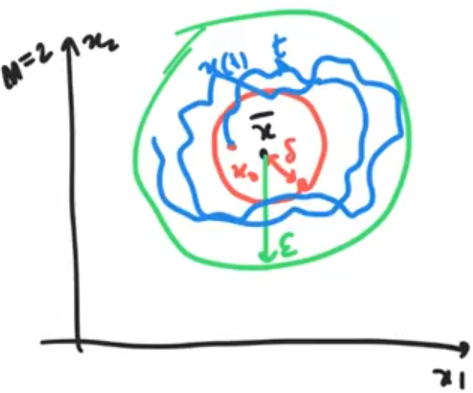
\includegraphics[width = \picwid]{traiettoria_stabile}
\end{figure}

Invece per la asintoticamente stabilità si ha la seguente traiettoria
\begin{figure}[h]
\centering
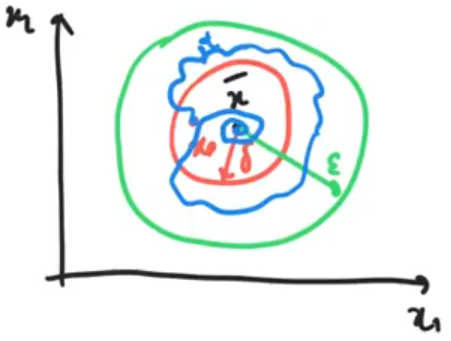
\includegraphics[width=\picwid]{traiettoria_asintoticamente_stabile}
\end{figure}

Un punto di equilibrio è invece instabile se non è stabile.

\newpage
\subsubsection{Esempio stabilità sistema del primo ordine}
Si consideri per semplicità un sistema del primo ordine, può essere
rappresentata la sua equazione caratteristica
$\dot{x} = f(x,\overline{u})$, il punto di stabilità si individua mediante
l'intersezione con l'asse delle ascisse $(\dot{x}=0)$. Si individua su questo
asse l'intorno $\overline{x} \pm \varepsilon$,
si applica una perturbazione $\delta$ spostando il punto di equilibrio, ad
esempio verso sinistra, ma a sinistra la derivata è positiva, dunque la $x$
tenderà nuovamente ad aumentare e ritornare nel punto di equilibrio, viceversa
se si analizza una perturbazione verso destra, la
derivata sarà negativa e quindi lo stato tenderà a diminuire nuovamente.
\begin{figure}[h]
\centering
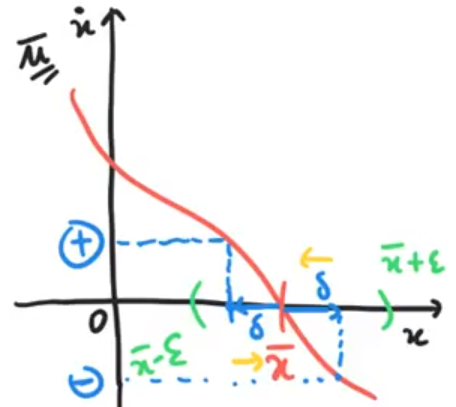
\includegraphics[width=\picwid]{equilibrio_stabile_1D}
\end{figure}
Se la curva fosse monotona decrescente, l'ampiezza $\varepsilon$ potrebbe
essere comunque grande, il sistema ritornerà sempre nel punto di
equilibrio.

Ciò potrebbe non essere vero, dunque è necessario definire la \textbf{Regione
di Asintotica Stabilità} o RAS il luogo delle traiettorie che ritornano sempre
nel punto di equilibrio.
$$
\text{RAS}(\overline{x})=\left\{ \stackrel{u=\overline{u}}{x_0\in X^n}
\ :\ \stackrel{t\to+\infty}{ x_0 \to \overline{x} }\right\}
$$
Nel caso in esame il RAS è tutto il dominio $\mathbb{R}$ dunque il punto
$\overline{x}$ viene definito globalmente asintoticamente stabile.
L'asintotica stabilità non dipende da $\delta$.

\newpage
\subsubsection{Funzione spezzata}
Si presenta una funzione definita da una spezzata come in figura.
Si individuano i punti di equilibrio
$$
\overline{x} = (-\infty,-1] \cup \{2,5\}
$$
Si vede, valutando il segno della derivata che il punto 2 ad esempio è
asintoticamente stabile per $\text{RAS}(2) = (-1,5)$.
Viceversa per il punto 5, qualunque sia la $\varepsilon$ scelta, la traiettoria
si allontanerà sempre dal punto di equilibrio dunque $\overline{x}=5$ è
instabile.
\begin{figure}[h]
\centering
\includegraphics[width=\picwid]{stabilità_spezzata}
\end{figure}
Nella regione  minore di -1 la derivata è nulla su un intero intervallo, dunque
esiste un'intera regione d punti di equilibrio, è verificata la proprietà di
stabilità ma non di asintotica stabilità, lo stato resta nello stesso punto
dopo essere stato perturbato.

Il punto -1 è instabile a causa della pendenza positiva della funzione a destra.

\subsection{Stabilità nei sistemi lineari e stazionari}
Si scrive il sistema nella forma lineare di stato e ingresso, ponendo un
ingresso costante
$$
\dot{x} = Ax + Bu\quad u(t)=\overline{u}=\text{cost} :
0=A\overline{x}+B\overline{u}
$$
Si supponga che il sistema non sia omogeneo
$$
\overline{u}\neq0\left\langle
\begin{aligned}
\text{det}(A)\neq 0 &\Rightarrow \exists ! \text{ equilibrio}\ : \
\overline{x}=-A^{-1}B\overline{u} \\
\text{det}(A) = 0 & \left\langle
\begin{aligned}
B\overline{u} \in \text{Immagine}\{A\} &\Rightarrow \infty \text{ equilibri} :
\overline{\overline{x}} + x_{\text{ker}(A)}\\
B\overline{u} \notin \text{Immagine}\{A\} &\Rightarrow \nexists \text{
equilibrio}
\end{aligned}
\right.
\end{aligned}
\right.
$$

Se invece l'ingresso $\overline{u}$ è nullo si risolvono i seguenti due casi
$$
\overline{u}=0\Rightarrow(A\overline{x}=0) \left\langle
\begin{aligned}
\text{det}(A) \neq 0 & \Rightarrow \exists! \text{ equilibrio} :
\overline{x}=0\\
\text{det}(A) = 0 & \Rightarrow \exists \infty \text{ equilibri} :
\overline{x} \in \text{Ker}(A)
\end{aligned}\right.
$$

\newpage
\subsubsection{Analisi di un punto di equilibrio}
Si scelga un punto di equilibrio qualsiasi
$(\overline{x},\overline{u})$ se il sistema è in equilibrio vale l'equazione di
Lagrange, ricordando che il punto iniziale è pari allo stato in cui si trova il
sistema in quel momento
$$
\overline{x} = e^{At} \overline{x} + \int_0^t e^{a(t-\tau)} B\overline{u}d\tau
$$
si perturba lo stato
$$
x(t) = e^{At}(\overline{x}+\Delta x)+ \int_0^t e^{a(t-\tau)} B\overline{u}d\tau
$$
Si valuta la differenza tra lo stato dopo la perturbazione e prima,
accertandosi che la norma della differenza sia minore di $\varepsilon$
$$
x(t)-\overline{x} = e^{At}\Delta x
\longrightarrow ||x(t)-\overline{x}|| =
||e^{At}\Delta x|| < \varepsilon
$$
Nella norma non compaiono il punto di equilibrio e lo stato iniziale, dunque la
stabilità del punto di equilibrio dipende solo dalla matrice $A$ e dalla
perturbazione $\Delta x$, se un solo punto di equilibrio è stabile, allora lo
saranno tutti. Questa affermazione vale solo per i sistemi lineari e non quelli
non lineari, un chiaro esempio è il pendolo analizzato precedentemente che ha
un punto stabile ed uno instabile ma non è un sistema lineare.

Le funzioni del tempo contenute nella matrice esponenziale $e^{At}$ sono i
\textit{modi naturali}, se questi sono limitati nel tempo, allora la norma sarà
sicuramente limitata. I modi dipendono però dagli autovalori della matrice $A$
$$
A = \left\{\begin{aligned}
\Re{\lambda_i}&<0 \ \forall i & &\Leftrightarrow \text{Sistema asintoticamente
stabile}\\
\Re{\lambda_i} &\leq 0 \ \forall i &
&\stackrel{\Re\{\lambda_j\}=0\Rightarrow m_{aj}=m_{gj}}{\Rightarrow}
\Rightarrow \text{Sistema stabile, i modi sono limitati}\\
\text{Altri } &\text{casi } & & \text{Sistema instabile}
\end{aligned}
\right.$$

Si è capito che al fine di analizzare la stabilità di un sistema è sufficiente
conoscere le radici del suo polinomio caratteristico. Non sempre è però facile
calcolare le radici di un polinomio se questo è di ordine superiore al secondo.


\subsection{Criterio di Routh-Hurwitz}
Al fine di verificare la asintotica stabilità di un sistema è però necessario
solo calcolare il segno della parte reale delle radici e non il loro valore
esatto, per fare ciò è comodo utilizzare il criterio di Routh,
composto da una condizione necessaria ed una necessaria e sufficiente.
\begin{itemize}
\item Condizione necessaria: i coefficienti del polinomio sono tutti dello
stesso segno (per $n\leq2$ è anche sufficiente)
\item Condizione sufficiente: la tabella di Routh-Hurwitz è ben definita e
tutti i coefficienti della prima colonna devono avere lo stesso segno
\end{itemize}

Sia $P(\lambda)$ un polinomio caratteristico
$$
P(\lambda) = \alpha_ns^n + \alpha_{n-1}s^{n-1} + \ldots + \alpha_0
$$
si costruisce la seguente tabella di Routh con $n+1$ righe, si dispongono
nelle prime due righe i coefficienti del polinomio, il resto delle righe sono
nulle.

\begin{table}[h]
$$
\begin{array}{c|ccccc}
 n & \alpha_n & \alpha_{n-2} & \alpha_{n-4} & \cdots \\
 n-1 & \alpha_{n-1} & \alpha_{n-3} & \cdots & \cdots \\ \hline
 n-2 & c_{n-2,1} & c_{n-2,2} & \cdots & \cdots \\
 n-3 & c_{n-3,1} & c_{n-3,2} & \cdots & \cdots\\
 \vdots \\
 0 & c_{0,1}
\end{array}
$$
\caption{Tabella di Routh}
\label{tab:tabella_routh}
\end{table}
Il generico coefficiente $c_{i,k}$ si ottiene
$$
c_{i,k} = -\frac{1}{c_{i+1,1}}\begin{vmatrix}
c_{i+2,1} & c_{i+2,k+1} \\
c_{i+1,1} & c_{i+1,k+1}
\end{vmatrix}
$$
Gli elementi nella prima colonna nel determinante sono sempre gli stessi e non
dipendono dalla colonna $k$ in cui si sta calcolando il coefficiente.

Se la prima colonna della tabella \ref{tab:tabella_routh} contiene tutti numeri
diversi da zero allora la tabella si definisce ben definita.
Il numero di radici a parte reale negativa è pari al numero di permanenze di
segno nella tabella, ossia il numero di volte in cui si contano due numeri
consecutivi con lo stesso segno.
Il numero di radici a parte reale negativa è pari al numero di permanenze di
segno della prima colonna della matrice, viceversa quelle a parte positiva sono
pari alle differenze di segno tra due valori consecutivi nella colonna.
Può essere utile capire il numero di radici positive al fine di correggere
eventualmente il sistema.

\newpage
\subsubsection{Esempio numerico}
Si consideri il seguente polinomio
$$
P(s) = s^4+6s^3 + 13s^2 + +12s +4
$$
La condizione necessaria è verificata, tutti i coefficienti sono positivi, si
costruisce la tabella di Routh.
\begin{table}[h]
$$
\begin{array}{c|ccc}
4 & 1 & 13 & 4\\
3 & 6 & 12 \\ \hline
2 & 11 & 4 \\
1 & 108 & & (\times11)\\
0 & 4
\end{array}
$$
\end{table}
Si calcolano i coefficienti
$$
c_{2,1} = -\frac{1}{6}\begin{vmatrix}
1 & 13\\
6 & 12
\end{vmatrix} = 11
$$
$$
c_{2,2} = -\frac{1}{6}\begin{vmatrix}
1 & 4\\
6 & 0
\end{vmatrix} = 4
$$
In questo caso è presente lo zero nella matrice, il coefficiente $c_{2,2}$ è
proprio pari al termine presente nella posizione
$c_{4,3}$ ovvero 4, non è necessario calcolare il determinante.
$$
c_{1,1} = -\frac{1}{11}\begin{vmatrix}
6 & 12 \\
11 & 4
\end{vmatrix} = \frac{108}{11}
$$
Si può moltiplicare per qualunque scalare positivo un'intera riga senza
alterare il risultato, si può moltiplicare la riga 1 per 11.
Anche il termine $c_{0,1}$ assume direttamente il valore 4, senza calcolare il
determinante.
La matrice è ben definita, sono presenti quattro permanenze di segno, il
polinomio ha tutte radici a parte reale negativa. Il polinomio si poteva
infatti riscrivere come
$$
p(s) = (s+1)^2(s+2)^2
$$
